The European Organization for Nuclear Research (CERN\footnote{The name CERN is derived from the acronym for the French Conseil Europ\'{e}en pour la Recherch Nucl\'{e}aire}) was founded in 1954 and is based in the suburb of Geneva on the Franco\textendash Swiss border.
The main function of CERN is to provide particle accelerators and detectors for high-energy physics research.
The physicists and engineers at CERN are probing the fundamental structure of the universe using the world's largest and most complex scientific facility \textemdash \ the Large Hadron Collider (LHC)~\cite{1748-0221-3-08-S08001}.
In the LHC, the particles are boosted to high energies and collide at close to the speed of light.
The results of the collisions are recorded by the various detectors.
There are seven experiments at the LHC.
The biggest of these experiments are ATLAS (A Toroidal LHC ApparatuS)~\cite{1748-0221-3-08-S08003} and CMS (Compact Muon Solenoid)~\cite{1748-0221-3-08-S08004} which use general-purpose detectors to investigate a broad physics programme ranging from the search for the Higgs boson to extra dimensions and particles that could make up dark matter.
The ALICE (A Large Ion Collider Experiment)~\cite{1748-0221-3-08-S08002} experiment is designed to study the physics of quark-gluon plasma form and the LHCb (Large Hadron Collider beauty)~\cite{1748-0221-3-08-S08005} experiment specializes in investigating of CP violation by studying the $b$-quark.
These four detectors sit underground in huge caverns of the LHC ring.
The rest three experiments, TOTEM~\cite{1748-0221-3-08-S08007}, LHCf~\cite{1748-0221-3-08-S08006}, and MoEDAL~\cite{Pinfold:1181486}, are smaller.
The TOTEM (TOTal Elastic and diffractive cross section Measurement)~\cite{1748-0221-3-08-S08007} experiment aims at the measurement of total cross section, elastic scattering, and diffractive dissociation.
The LHCf (Large Hadron Collider forward)~\cite{1748-0221-3-08-S08006} experiment is intended to measure the neutral particle produced by the collider using the forward particles.
The prime motivation of the MoEDAL (Monopole and Exotics Detector at the LHC)~\cite{Pinfold:1181486} experiment is to search directly for the magnetic monopole.

\section{The Large Hadron Collide}

The LHC~\cite{1748-0221-3-08-S08001} is the world's largest and most powerful accelerator which accelerates and collides protons in a 26.7 km circumference crossing the Franco\textendash Swiss border 100 m underground.
Built in the tunnel of the former LEP (Large Electron\textendash Positron), the LHC is capable of colliding protons as well as heavy ions.
Comparing with the LEP which collides electrons and positrons, the advantage of the LHC is the lower energy loss \footnote{The energy loss for protons is about eleven orders of magnitude smaller than the electrons} in the synchrotron radiation, such that higher energies can be reached by the LHC.
The LHC is designed for collisions at a centre-of-mass energy $\sqrt{s}=14$ TeV and an instantaneous luminosity of $\mathcal{L} =10^{34} \ \textrm{cm}^{-2}\textrm{s}^{-1}$.
Figure~\ref{fig:CERN_accelerator_complex} shows the infrastructure of the LHC and the pre-accelerator system.

\begin{figure}[htbp]
\begin{center}
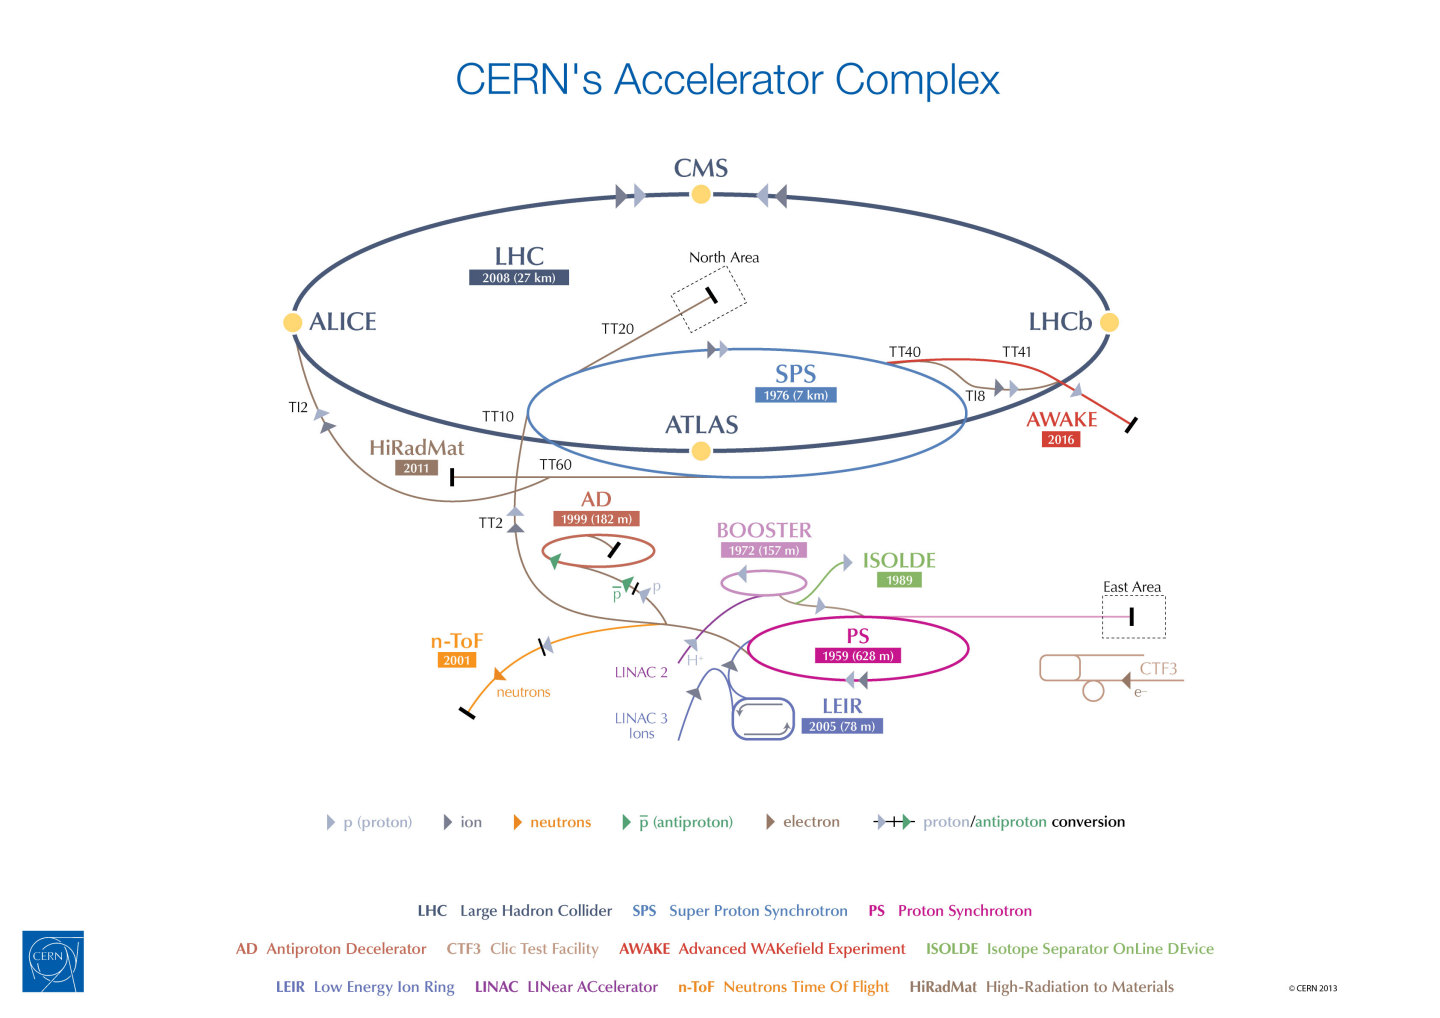
\includegraphics[scale=0.5]{CERN's-accelerator-complex2013.jpg}
\caption{The accelerator complex at CERN~\cite{Marcastel:1621583}.}
\label{fig:CERN_accelerator_complex}
\end{center}
\end{figure}

The protons are extracted by ionization from a hydrogen source and are accelerated to 50 MeV by the linear accelerator LINAC2.
Then they are injected into the Proton Synchrotron Booster (PSB) where the proton energies are increased to 1.4 GeV before they enter the Proton Synchrotron (PS) which accelerates the protons to 25 GeV.
Next, the proton energies are increasing to 450 GeV in the Super Proton Synchrotron (SPS). 
Finally, the protons are split into two beams and enter the LHC where the two beams run in two adjacent beam pipes with opposite directions.
In order to keep the protons on the circular trajectory in the LHC, 1232 superconducting dipole magnets~\cite{1288863} generate a magnetic field strength of 8.33 T to bend the proton beams in eight arcs.
Additionally, 392 quadrupole magnets~\cite{1288863} are installed to focus the beam.
A cryogenic system running with super-fluid helium-4 is used to cool down the superconducting magnets to a temperature of 1.7 K.

For a given physics process, the event rate is proportional to the cross section $\sigma$ of this process.
\begin{equation}
\frac{dN}{dt} = \mathcal{L}\cdot\sigma
\end{equation}
where $N$ is the number of events and $\mathcal{L}$ denotes the luminosity of the beam.
The luminosity of the beam, $\mathcal{L}$ can be calculated by
\begin{equation}
\mathcal{L} = \frac{N^{2} f}{4 \pi \sigma_{x} \sigma_{y}} \cdot F
\end{equation}
where $N$ is the number of protons, $f$ is the bunches crossing frequency, and the $\sigma_{x}$ and $\sigma_{y}$ are the $x$ and $y$ components for cross section $\sigma$.
The geometric luminosity reduction factor, $F$, is related to the crossing angle at the Interaction Point (IP).
Considering a beam consisting of $1.15 \times 10^{11}$ protons with bunching spacing of 25 ns, the transversal size of the bunch at Interaction Pointe $16\times 10^{-4}$ cm, and taking the geometric luminosity reduction factor as 1, the design luminosity of $10^{34}$ cm$^{-2}$s$^{-1}$ can be reached.

The first beam was circulated through the collider on the morning of 10 September 2008~\cite{CERN-COURIER-Sep192008}.
However, a magnet quench incident occurred on 19 September 2008 and caused extensive damage to over 50 superconducting magnets, their mountings, and the vacuum pipe.
Most of 2009 was spent on repairs the damage caused by the magnet quench incident and the operations resumed on 20 November of that year.
The first phase of data-taking (Run 1) started at the end of 2009 and the beam energy was increased to a centre-of-mass $\sqrt{s}=7$ TeV in 2011 and $\sqrt{s} = 8$ TeV in 2012.
The total integrated luminosity of 5.46 fb$^{-1}$ was collected in 2011 and of 22.8 fb$^{-1}$ was collected in 2012.
Since 13 February 2013 the LHC was in the Long Shutdown 1 (LS1) phase for maintenance and upgrades.
On 5 April 2015, the LHC restarted and was operating at a centre-of-mass energy $\sqrt{s}=13$ TeV throughout the Run 2 phase\footnote{The Run 2 data-taking started from 2015}.


%%%%%
%%%%%
%%%%%

\section{The ATLAS experiment}

The ATLAS\footnote{A Toroidal LHC Apparatus} detector is a multi-purpose detector housed in its cavern at point 1 at the LHC.
It is the largest experiment at the LHC with a length of 44 m, a diameter of 25 m, and a weight of approximately 7 000 tonnes.
It consists of three high precision sub-detector systems which are arranged concentrically around the interaction point and in forward and backward symmetrically.
Related to this symmetry, the ATLAS detector is sectioned into the central barrel region with one end-cap region perpendicular to the beam pipe on either side.
Figure~\ref{fig:ATLAS_detector} shows an overview of the ATLAS detector with its major components.

\begin{figure}[htbp]
\begin{center}
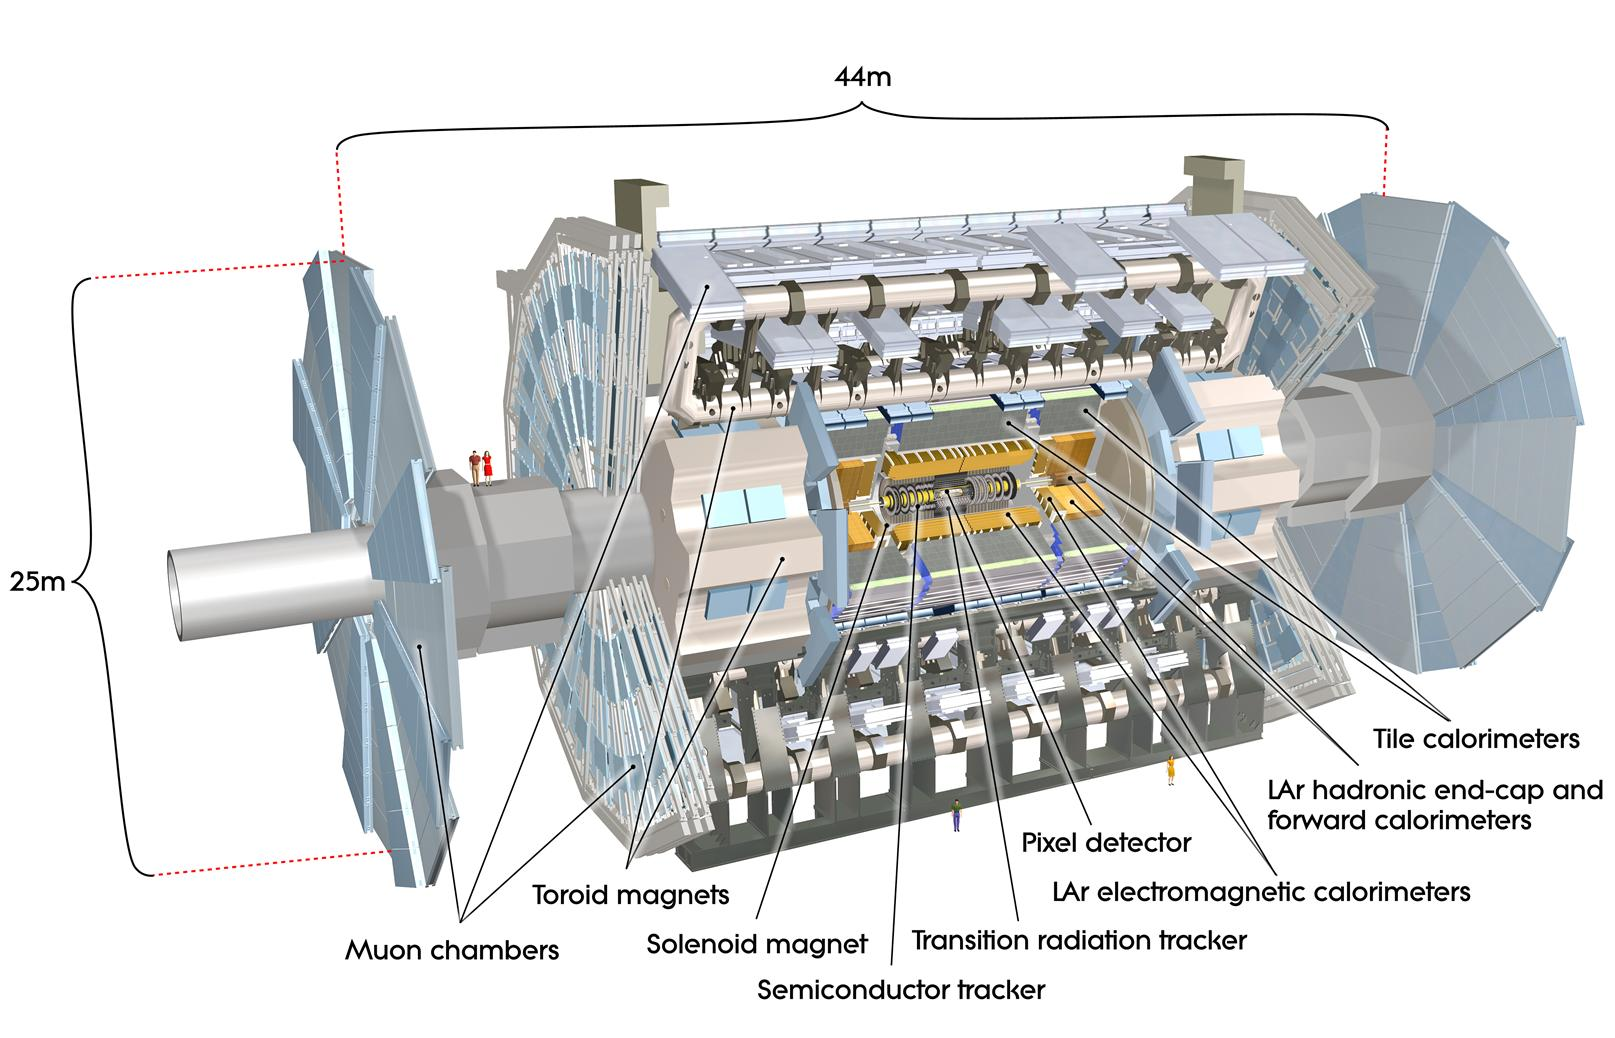
\includegraphics[scale=0.5]{0803012_01-A4-at-144-dpi.jpg}
\caption{Overview of the ATLAS detector}
\label{fig:ATLAS_detector}
\end{center}
\end{figure}

The ATLAS detector is designed to record the proton-proton interactions delivered by the LHC.
It can identify particles and measure their tracks and energies with very high precision, therefore, it is sensitive to large areas of particle physics phenomena from the precision measurement of the Standard Model (SM) to beyond the SM.
The detector is constituted by three sub-detector systems and the magnet system.
The innermost part of the detector is called the inner detector which identifies and reconstructs the charged particles as well as the primary and secondary vertices.
Around it, the calorimeter system is built as a cylindrical barrel with caps at each end to measure the particle energies.
The detector is completed by the muon spectrometer which performs identification and measurement of momenta of muons.
The magnetic system produces a field of B = 0.5 T and B = 1 T at barrel and two end-cap, respectively.
The detector has to withstand large collision rates with approximately 1000 particles per collision, therefore, a fast readout and a three-level trigger system are implemented to reduce the event rate from 40 MHz to 200 Hz.
The ATLAS coordinate system and the detail of each sub-detector systems are described in the following sections.

\subsection{The ATLAS coordinate system}

ATLAS uses a right-handed coordinate system with its origin at the nominal proton-proton interaction point (IP) in the centre of the detector and the $z$-axis along the beam pipe.
Along the $z$-axis the detector is divided into side-A (positive $z$) and side-C (negative $z$).
The positive $x$-axis is defined by the direction pointing from the IP to the centre of the LHC ring, and the positive $y$-axis points upward.%Cylindrical coordinates $(r, \phi)$ are used in the transverse plane.
The azimuthal angle $\phi$ is measured around the beam pipe  and the polar angle $\theta$ is the angle from the $z$-axis.
The transverse momentum $p_{\mathrm{T}}$, the transverse energy $E_{\mathrm{T}}$ and the missing transverse
energy $E_{\mathrm{T}}^{\mathrm{miss}}$ are defined in the transverse plane\footnote{$x-y$ plane}, here exemplary for $p_{\mathrm{T}}$:
%
\begin{equation}
p_{\mathrm{T}}= \sqrt{p_{x}^{2} + p_{y}^{2}}
\end{equation}
%
An important quantity in hadron collider physics is the \textbf{rapidity}, $y$, because of the invariance $y$ under Lorentz boosts in the longitudinal direction.
The rapidity is defined as
%
\begin{equation}
y = \frac{1}{2} \ln\Big[\frac{E + p_{z}}{E - p_{z}}\Big]
\end{equation}
%
where $E$ denotes the particle energy and $p_{z}$  is the component of the momentum along the beam direction.
Since mainly leptons can be considered massless in respect to the nominal centre-of-mass energy, the pseudorapidity, $\eta$, is used in stead of using the $y$.
For a massless particle, the \textbf{pseudorapidity}, $\eta$, depends on the polar angle $\theta$ through:
%
\begin{equation}
\eta = - \ln \tan \frac{\theta}{2}
\end{equation}
%
For a particle with the energy $E$ much larger than its mass, the approximation $E \approx |\vec{p}|$ is valid.
The distance, $\Delta R$, between two objects in the $\eta-\phi$ plan is given by
%
\begin{equation}
\Delta R = \sqrt{\Delta \eta^{2} + \Delta \phi^{2}}
\end{equation}
%
where $\Delta \eta$ and $\Delta \phi$ are the difference in pseudorapidity and azimuthal angle, respectively.

\subsection{The Inner Detector and Tracking System}
%\subsubsection{Pixel Detector}
%\subsubsection{Semi Conductor Tracker}
%\subsubsection{Transition Radiation Tracker}
%\subsubsection{Solenoid Magnet}

\subsection{The Calorimeter}
%\subsubsection{Electromagnetic Calorimeter}
%\subsubsection{Hadronic Calorimeter}
%\subsubsection{Forward Calorimeter}

\subsection{The Muon Spectrometer}

The outermost part of the ATLAS detector is the Muon Spectrometer~\cite{1748-0221-3-08-S08003}~\cite{Palestini:681459}~\cite{0910.2767}.
Muons have the same properties as electrons but 200 times heavier than the electrons and muons don't interact predominately by Bremsstrahlung but have minimal ionizing at LHC energy in the inner layers of the detector.
Only the muons with an energy less than 5 GeV are stopped before the Muon Spectrometer.
Therefore, muons are the only measurable particles that can penetrate the Inner Detector and the Calorimeters.
In order to determine the muon momentum with high precision, a detector that concentrates on the measurement of muons is necessary.

The Muon Spectrometer is designed to measure the transverse momentum ($p_{\mathrm{T}}$) of muons with $p_{\mathrm{T}} > 3$ GeV with a resolution of 3\% for $p_{\mathrm{T}} < 250$  GeV and increasing to 10\% at 1 TeV.
It consists of large toroid magnets system and three layers of high precision tracking chambers which allow a precise measurement of the muon momentum over nearly the full solid angle.
The barrel toroid magnet system is composed of eight superconducting coils which are installed radial symmetrically around the beam pipe.
It covers the range $|\eta| < 1.4$ and bends the trajectories of muons with the bending power 1.5 to 5.5 Tm.
The magnetic field produced by the barrel toroid magnets provides an approximately 1~T field at the center of each coils, but is rather non-uniform, especially in the barrel-endcap transition region.
In the endcap toroid magnets system, the magnetic field is provided by eight superconducting coils, closed in an insulation vessel extending to about 10 m in diameter, located between the first and the second station of tracking chambers.
The endcap toroid magnets cover $1.6 < |\eta| < 2.4$ and provide a a magnetic field in the range of 1 to 2 T with bending power 1 to 7.5 Tm.

The Monitored Drift Tubes (MDTs) consists of cylindrical drift tubes, filled with a gas mixture of argon and carbon dioxide.
A tungsten-rhenium alloyed aluminium wire in the centre of each tube collects the electrons freed by ionization of the gas volume by traversing muons.
The MDTs covers a full range of $|\eta| < 2.7$, while the inner layer only covers $|\eta| < 2.0$.
The Cathode Strip Chambers (CSCs) provides a coverage range $2.0 < |\eta| < 2.7$, where MDTs would have occupancy problems.
Both MDTs and CSCs are used for precision tracking in the spectrometer bending plane and end-cap inner layer, respectively.
The Resistive Plate Chambers (RPCs) and Thin Gap Chambers (TGCs) are used for triggering in barrel and end-cap, they have sufficient intrinsic time resolution of 1.5 ns and 4 ns, respectively.
A sketch of the Muon Spectrometer and its four components are depicted in Figure~\ref{fig:muon_spectrometer} and Table~\ref{tab:muon_spectrometer_components} gives a summary of the Muon Spectrometer components

\begin{figure}[htbp]
\begin{center}
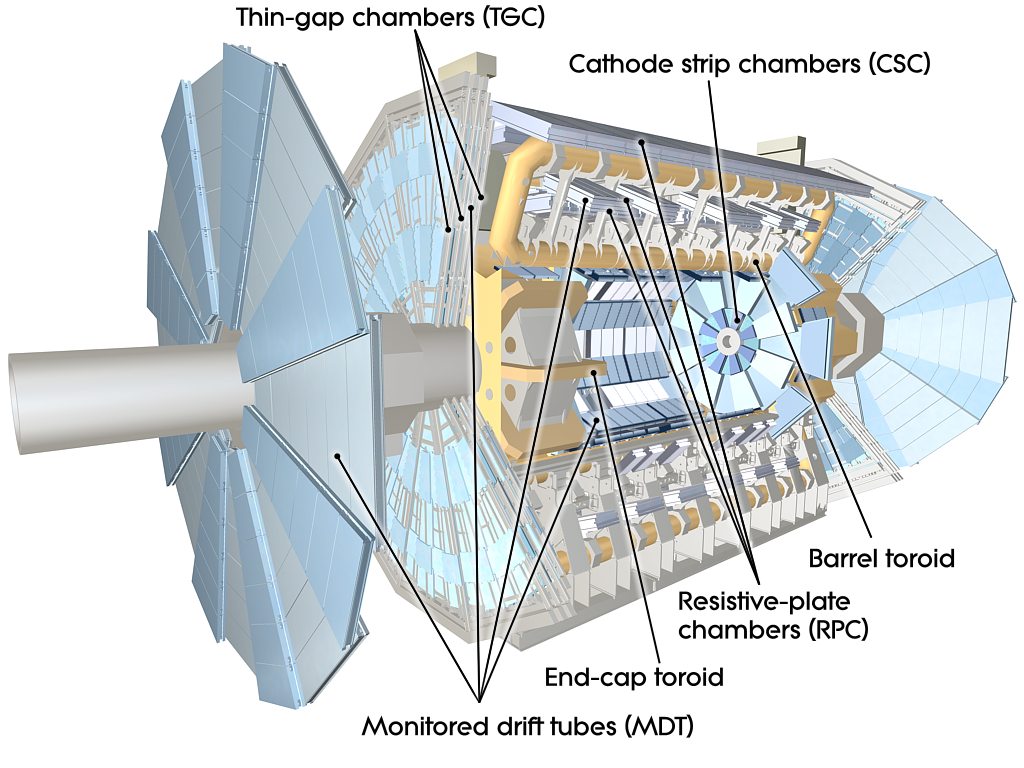
\includegraphics[scale=0.4]{MuonSystem_d3.png}
\caption{Sketch of the muon system of the ATLAS detector~\cite{1748-0221-3-08-S08003}.}
\label{fig:muon_spectrometer}
\end{center}
\end{figure}

\begin{table}[htbp]
\begin{center}
\begin{tabular}{ccccc}
\hline
\hline
Type & Purpose & Location & $\eta$ coverage & Channel\\
\hline
MDT & Tracking & barrel + end-cap & $0.0 < \eta < 2.7$ & 354k\\
CSC & Tracking & end-cap layer 1 & $2.0 < \eta < 2.7$ & 30.7k\\
RPC & Trigger & barrel & $0.0 < \eta < 1.0$ & 373k\\
TGC & Trigger & end-cap & $1.0 < \eta < 2.4$ & 318k\\
\hline
\hline
\end{tabular}
\end{center}
\caption{A summary of the Muon Spectrometer components.}
\label{tab:muon_spectrometer_components}
\end{table}%



   
   
   
   



%The Muon Spectrometer is the outermost part of the ATLAS detector. Besides muons all particles that can be observed by the ATLAS detector are absorbed in the layers between the Inner Detector and the Muon Spectrometer, the calorimeters (see the following section). Muons are the only measurable particles that can penetrate all layers of the detector, thus escaping the detector without being stopped. This observation is a result of the underlying interaction mechanism of muons with the detector material. In principle, muons are leptons, as electrons, but 200 times heavier and therefore not interacting predominately by Bremsstrahlung, but by ionisation leaving only little energy in the inner layers of the detector.
%Consisting of three layers of high precision tracking chambers and large toroid magnets the Muon Spectrometer supplies a complementary measurement of the muon momentum and charge compared to the Inner Detector. Different types of ionisation chambers are used for detection: Monitored Drift Tubes (MDT), Cathode Strip Cham-bers (CSC), Resistive Plate Chambers (RPC) and Thin Gap Chambers (TGC). The acceptance range in pseudorapidity is |η| < 2.7. The relative resolution in transverse momentum in the Muon Spectrometer is 10 \% for 1 TeV muons.



%The central part of the muon momentum measurement are the barrel toroid magnet, covering the range |η| < 1.4, and the two smaller end-cap toroid magnets, covering 1.6 < |η| < 2.7. This configuration causes a bending of the trajectories of muons in the (r,z) plane rather than in (r,φ). In combination with three cylindrical layers of muon chambers and three layers of planes of chambers, perpendicular to the beam axis, this allows for a precise measurement of the muon momentum over nearly the full solid angle. The barrel layers consists of drift tubes for precision tracking, and resistive plate chambers with very fast response for triggering. The end-cap uses drift tubes and cathode strip chambers for precision tracking and thin gap chambers for triggering.



%The outermost part of the ATLAS detector is equipped by the muon spectrometer (MS) which concentrates on the measurement of muons. Due to the fact, that muons are minimal ionising at LHC energies, they traverse the detector without only little interactions. Only muons with an energy of less than 5 GeV are stopped before the MS. Nevertheless, to determine the muon momentum with high precision a specialised detector is necessary. Therefore, a toroid magnet system composed of eight superconducting coils which generates an almost circular field is installed radial symmetrically around the beam pipe. The muons are bent on curved trajectories whereby the bending power of the 0.5 T barrel field (|η| < 1.4) is 1.5-5.5 Tm and 1-7.5 Tm in the end-caps (1.6 < |η| < 2.4). The latter is provided by a magnetic field of 1 T. In the intermediate region both fields overlap. A sketch of the MS and its three sub-detectors is depicted in Figure 3.5.
%The middle and the outer layer of the Monitored Drift Tube Chambers (MDTs) extend over a full range of |η| < 2.7, while the inner layer covers only pseudorapidities smaller than 2.0. The MDT consists of cylindrical drift tubes, filled with a gas mixture of argon and carbon dioxide. A tungsten-rhenium alloyed aluminium wire in the centre of each tube collects the electrons freed by ionisation of the gas volume by traversing muons. Within a region of 2.0 < |η| < 2.7 Cathode Strip Chambers (CSCs) are applied to provide a better time resolution. Multi-wire proportional chambers with tungsten-rhenium anode wires are filled with a gas mixture as well, but the composition differs from the MDTs, i.e. 50 % carbon dioxide, 30 % argon and 20 % carbon tetra-fluoride is used.
%Both detectors are too slow to be used by the trigger. Only the Restrictive Plate Chambers (RPCs) and the Thin Gap Chambers (TGCs) have a sufficient intrinsic time resolution of 1.5 ns and 4 ns, respectively. A high electric field is applied in the 2 mm gap between the two parallel arranged restrictive plates of the RPC, such that a muon which enters the detector ionises the volume and causes avalanching. The collected signal can be exploited to veto fake muons, e.g. muons from cosmic rays, in the barrel region by a coincidence measurement. The end-caps are equipped by TGCs which operate similar to the multi- wire proportional chamber but with a radial and azimuthal segmentation of the wires to provide a good trigger signal.




\subsection{The Trigger System and Data Acquisition}

\subsection{}